\documentclass[tikz,border=10pt]{standalone}
\usepackage{tikz}
\usetikzlibrary{positioning, calc, arrows.meta, fit}

\begin{document}
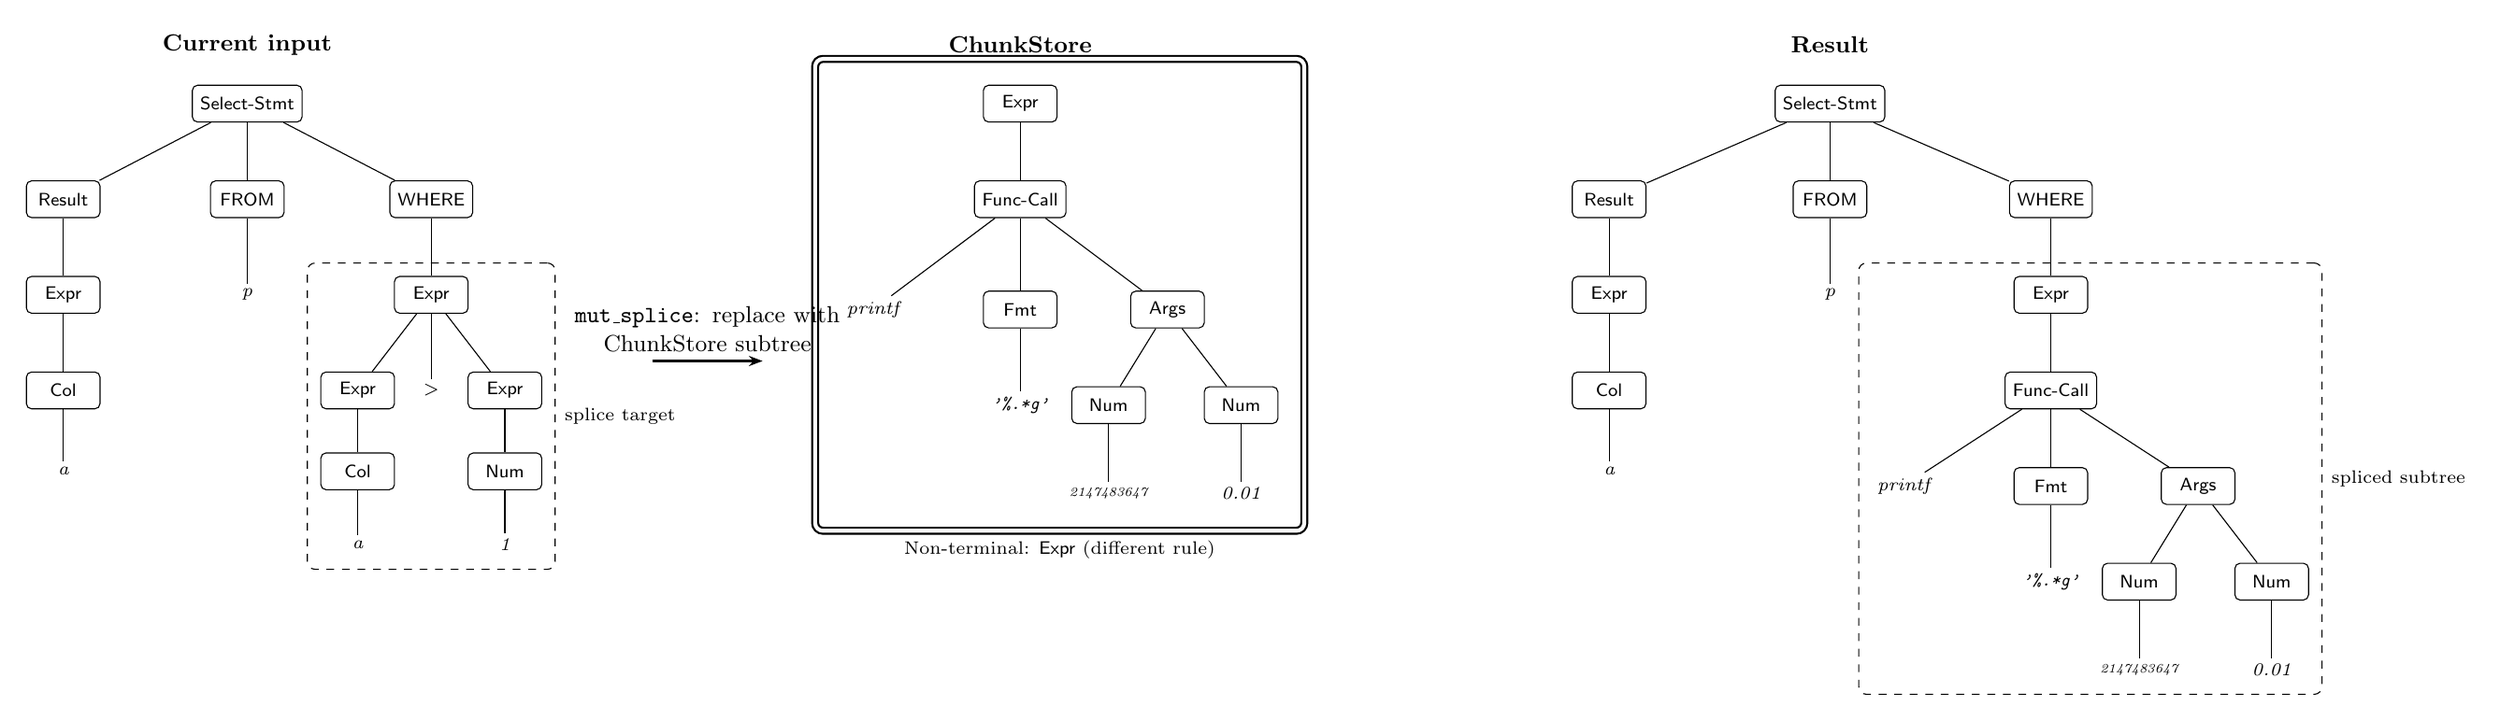
\begin{tikzpicture}[
    every node/.style={font=\small},
    % Non-terminal: small rounded rectangle, thin border
    nterm/.style={rectangle, rounded corners=2pt, draw=black, thin,
        minimum height=0.5cm, minimum width=1.0cm,
        inner sep=3pt, font=\scriptsize\sffamily},
    % Terminal: italic, no border
    term/.style={font=\scriptsize\itshape, inner sep=2pt},
    % Edge style
    edge/.style={thin},
    % Dashed highlight box
    highlight/.style={draw=black, dashed, thick, rounded corners=3pt,
        inner sep=5pt, thin},
    % ChunkStore box: double border
    chunkstore/.style={rectangle, draw=black, double, double distance=1.5pt,
        thick, rounded corners=3pt, inner sep=10pt},
    % Arrow between sections
    mutarrow/.style={-{Stealth[scale=0.8]}, thick},
]

% ====================================================
% SECTION 1: Current input (left)
% Tree: SELECT a FROM p WHERE a > 1
% ====================================================
\begin{scope}[shift={(0,0)}]

    % Section label
    \node[font=\small\bfseries] at (0, 0.8) {Current input};

    % Root
    \node[nterm] (L-root) at (0, 0) {Select-Stmt};

    % Level 1
    \node[nterm] (L-result) at (-2.5, -1.3) {Result};
    \node[nterm] (L-from) at (0, -1.3) {FROM};
    \node[nterm] (L-where) at (2.5, -1.3) {WHERE};

    % Level 2
    \node[nterm] (L-expr1) at (-2.5, -2.6) {Expr};
    \node[term] (L-p) at (0, -2.6) {p};
    \node[nterm] (L-expr2) at (2.5, -2.6) {Expr};

    % Level 3 (left branch)
    \node[nterm] (L-col1) at (-2.5, -3.9) {Col};

    % Level 3 (right branch: comparison)
    \node[nterm] (L-expr3) at (1.5, -3.9) {Expr};
    \node[term] (L-gt) at (2.5, -3.9) {$>$};
    \node[nterm] (L-expr4) at (3.5, -3.9) {Expr};

    % Level 4
    \node[term] (L-a1) at (-2.5, -5.0) {a};
    \node[nterm] (L-col2) at (1.5, -5.0) {Col};
    \node[nterm] (L-num) at (3.5, -5.0) {Num};

    % Level 5
    \node[term] (L-a2) at (1.5, -6.0) {a};
    \node[term] (L-1) at (3.5, -6.0) {1};

    % Edges
    \draw[edge] (L-root) -- (L-result);
    \draw[edge] (L-root) -- (L-from);
    \draw[edge] (L-root) -- (L-where);
    \draw[edge] (L-result) -- (L-expr1);
    \draw[edge] (L-from) -- (L-p);
    \draw[edge] (L-where) -- (L-expr2);
    \draw[edge] (L-expr1) -- (L-col1);
    \draw[edge] (L-expr2) -- (L-expr3);
    \draw[edge] (L-expr2) -- (L-gt);
    \draw[edge] (L-expr2) -- (L-expr4);
    \draw[edge] (L-col1) -- (L-a1);
    \draw[edge] (L-expr3) -- (L-col2);
    \draw[edge] (L-expr4) -- (L-num);
    \draw[edge] (L-col2) -- (L-a2);
    \draw[edge] (L-num) -- (L-1);

    % Dashed rectangle around the Expr subtree (splice target)
    \node[highlight, fit=(L-expr2)(L-expr3)(L-gt)(L-expr4)(L-col2)(L-num)(L-a2)(L-1),
        label={[font=\scriptsize, anchor=west]right:splice target}] (L-box) {};

\end{scope}

% ====================================================
% SECTION 2: ChunkStore (center)
% ====================================================
\begin{scope}[shift={(10.5,0)}]

    % Section label
    \node[font=\small\bfseries] at (0, 0.8) {ChunkStore};

    % Tree inside chunk store
    \node[nterm] (C-expr) at (0, 0) {Expr};
    \node[nterm] (C-func) at (0, -1.3) {Func-Call};

    \node[term] (C-printf) at (-2.0, -2.8) {printf};
    \node[nterm] (C-fmt) at (0, -2.8) {Fmt};
    \node[nterm] (C-args) at (2.0, -2.8) {Args};

    \node[term] (C-fmtv) at (0, -4.1) {\texttt{'\%.*g'}};
    \node[nterm] (C-int) at (1.2, -4.1) {Num};
    \node[nterm] (C-flt) at (3.0, -4.1) {Num};

    \node[term] (C-intv) at (1.2, -5.3) {\tiny 2147483647};
    \node[term] (C-fltv) at (3.0, -5.3) {0.01};

    % Edges
    \draw[edge] (C-expr) -- (C-func);
    \draw[edge] (C-func) -- (C-printf);
    \draw[edge] (C-func) -- (C-fmt);
    \draw[edge] (C-func) -- (C-args);
    \draw[edge] (C-fmt) -- (C-fmtv);
    \draw[edge] (C-args) -- (C-int);
    \draw[edge] (C-args) -- (C-flt);
    \draw[edge] (C-int) -- (C-intv);
    \draw[edge] (C-flt) -- (C-fltv);

    % ChunkStore double-border box
    \node[chunkstore, fit=(C-expr)(C-func)(C-printf)(C-fmt)(C-args)(C-fmtv)(C-int)(C-flt)(C-intv)(C-fltv)] (C-box) {};

    % Label below
    \node[font=\scriptsize, anchor=north] at (C-box.south)
        {Non-terminal: \textsf{Expr} (different rule)};

\end{scope}

% ====================================================
% SECTION 3: Result (right)
% Tree: SELECT a FROM p WHERE printf('%.*g', 2147483647, 0.01)
% ====================================================
\begin{scope}[shift={(21.5,0)}]

    % Section label
    \node[font=\small\bfseries] at (0, 0.8) {Result};

    % Root
    \node[nterm] (R-root) at (0, 0) {Select-Stmt};

    % Level 1
    \node[nterm] (R-result) at (-3.0, -1.3) {Result};
    \node[nterm] (R-from) at (0, -1.3) {FROM};
    \node[nterm] (R-where) at (3.0, -1.3) {WHERE};

    % Level 2
    \node[nterm] (R-expr1) at (-3.0, -2.6) {Expr};
    \node[term] (R-p) at (0, -2.6) {p};
    \node[nterm] (R-expr2) at (3.0, -2.6) {Expr};

    % Level 3 (left branch)
    \node[nterm] (R-col1) at (-3.0, -3.9) {Col};

    % Level 3 (right branch: spliced func-call)
    \node[nterm] (R-func) at (3.0, -3.9) {Func-Call};

    % Level 4
    \node[term] (R-a1) at (-3.0, -5.0) {a};
    \node[term] (R-printf) at (1.0, -5.2) {printf};
    \node[nterm] (R-fmt) at (3.0, -5.2) {Fmt};
    \node[nterm] (R-args) at (5.0, -5.2) {Args};

    % Level 5
    \node[term] (R-fmtv) at (3.0, -6.5) {\texttt{'\%.*g'}};
    \node[nterm] (R-int) at (4.2, -6.5) {Num};
    \node[nterm] (R-flt) at (6.0, -6.5) {Num};

    % Level 6
    \node[term] (R-intv) at (4.2, -7.7) {\tiny 2147483647};
    \node[term] (R-fltv) at (6.0, -7.7) {0.01};

    % Edges
    \draw[edge] (R-root) -- (R-result);
    \draw[edge] (R-root) -- (R-from);
    \draw[edge] (R-root) -- (R-where);
    \draw[edge] (R-result) -- (R-expr1);
    \draw[edge] (R-from) -- (R-p);
    \draw[edge] (R-where) -- (R-expr2);
    \draw[edge] (R-expr1) -- (R-col1);
    \draw[edge] (R-col1) -- (R-a1);
    \draw[edge] (R-expr2) -- (R-func);
    \draw[edge] (R-func) -- (R-printf);
    \draw[edge] (R-func) -- (R-fmt);
    \draw[edge] (R-func) -- (R-args);
    \draw[edge] (R-fmt) -- (R-fmtv);
    \draw[edge] (R-args) -- (R-int);
    \draw[edge] (R-args) -- (R-flt);
    \draw[edge] (R-int) -- (R-intv);
    \draw[edge] (R-flt) -- (R-fltv);

    % Dashed rectangle around the spliced subtree
    \node[highlight, fit=(R-expr2)(R-func)(R-printf)(R-fmt)(R-args)(R-fmtv)(R-int)(R-flt)(R-intv)(R-fltv),
        label={[font=\scriptsize, anchor=west]right:spliced subtree}] (R-box) {};

\end{scope}

% ====================================================
% ARROWS between sections
% ====================================================

% Arrow from Section 1 to Result
\draw[mutarrow] (5.5, -3.5) -- node[above, font=\small, align=center, text width=4cm]
    {\texttt{mut\_splice}: replace with\\ChunkStore subtree} (7.0, -3.5);

\end{tikzpicture}
\end{document}
